\documentclass{article}

\usepackage[short]{optidef}
\usepackage{amsmath}
\usepackage{amsthm}
\usepackage{gensymb}
\usepackage[a4paper]{geometry}
\usepackage{color}
\usepackage{graphicx}
\usepackage[labelfont=bf]{caption}
\usepackage{my-notation}
\usepackage{float}
\usepackage{mhchem}
\restylefloat{table}
\usepackage{appendix}
\usepackage{enumitem}

\newtheorem{theorem}{Theorem}[section]
\theoremstyle{example}
\newtheorem{exmp}{Example}[section]
\theoremstyle{definition}
\newtheorem{definition}{Definition}[section]
\theoremstyle{assumption}
\newtheorem{assumption}{Assumption}[section]
\theoremstyle{lemma}
\newtheorem{lemma}{Lemma}[section]

\graphicspath{{./images/}}
\title{Literature Notes}
\author{Brittany Hall}
\date{}

\begin{document}
	\maketitle
%%%%%%%%%%%%%%%%%%%%%%%%%%%%%%%%%%%%%%%%%%%%%%%%%%%%%%%%%%%%%%%%%%%%%%%
	\section{Numerical Optimal Control-Parametric Optimization}
%%%%%%%%%%%%%%%%%%%%%%%%%%%%%%%%%%%%%%%%%%%%%%%%%%%%%%%%%%%%%%%%%%%%%%%
%%%%%%%%%%%%%%%%%%%%%%%%%%%%%%%%%%%%%%%%%%%%%%%%%%%%%%%%%%%%%%%%%%%%%%%
	\subsection{Parametric NLPs}
	A generic non-linear programming problem can be written in the following way:
		\begin{mini!}
			{w}{\Phi(w,p))}{}{}
			\addConstraint{g(w,p)=0}{}
			\addConstraint{h(w,p)\leq0}{}
		\end{mini!}
		where $\vec{p}$ is a vector of parameters.
	Changes of active set yield non-smooth points in the solution manifold $w(p)$.
	It is important to understand that $w(p): p\in\mathbb{R}^p\rightarrow w\in\mathbb{R}^n$ as a genuine function defined by the parametric NLP.
	Solution $w$ is an implicit function of the parameters $p$ so we need to use IFT.
	\par
	When looking at problems like this, we consider four things:
	\begin{itemize}
		\item continuity and differentiability
		\item sensitivities $\frac{\partial w}{\partial p}$
		\item Predictors: using $w(p_0)$ what can I say about $w(p)$?
			\begin{equation*}
				w(p)\approx w(p_0)+\frac{\partial w}{\partial p}(p-p_0)
			\end{equation*}
		\item Path-following: how to keep track of $w(p)$ for a (continuously) changing $p$?
	\end{itemize}
%%THRM%%
\begin{theorem}
	If $w(p)$ fulfils LICQ and strict SOSC (positive definite Hessian), then $w(p)$ is continuous around $p$.
\end{theorem}
%%%%%%%%%%%%%%%%%%%%%%%%%%%%%%%%%%%%%%%%%%%%%%%%%%%%%%%%%%%%%%%%%%%%%%%
%%%%%%%%%%%%%%%%%%%%%%%%%%%%%%%%%%%%%%%%%%%%%%%%%%%%%%%%%%%%%%%%%%%%%%%
%%%%%%%%%%%%%%%%%%%%%%%%%%%%%%%%%%%%%%%%%%%%%%%%%%%%%%%%%%%%%%%%%%%%%%%
	\subsubsection{Differentiability}
%%THRM%%
\begin{theorem}
	Consider $w(p)$ at a given $p$ with
	\begin{itemize}
		\item LICQ and strict SOSC
		\item no weakly active constraint $h$
	\end{itemize}
	then $\nabla_pw(p)$ exists.
\end{theorem}
%%%%%%%%%%%%%%%%%%%%%%%%%%%%%%%%%%%%%%%%%%%%%%%%%%%%%%%%%%%%%%%%%%%%%%%
%%%%%%%%%%%%%%%%%%%%%%%%%%%%%%%%%%%%%%%%%%%%%%%%%%%%%%%%%%%%%%%%%%%%%%%
%%%%%%%%%%%%%%%%%%%%%%%%%%%%%%%%%%%%%%%%%%%%%%%%%%%%%%%%%%%%%%%%%%%%%%%
	\subsubsection{Sensitivity in Newton}
	\begin{itemize}
		\item Newton as an implicit function
			\begin{mini!}
				{w}{\Phi(w,p))}{}{}
				\addConstraint{g(w,p)=0}{}
			\end{mini!}
		Solution $w(p),\lambda(p)$ implicitly given by the KKT conditions:
			\begin{align*}
				\nabla_w\Lagrange(w,p\lambda)&=0\\
				g(w,p)&=0
			\end{align*}
			\begin{theorem}[Implicit Function Theorem]
				Let $z$ be implicitly given by the $\mathcal{C}^1$ function:
				\begin{equation*}
				R(z,p)=0 \text{ with } \nabla_zR(z,p_0) \text { full rank }
				\end{equation*}
				Then for any $p_0$ there is a $\mathcal{C}^2$ function $\xi(p)$ such that:
				\begin{equation*}
					R(\xi(p),p)=0
				\end{equation*}
				holds in a neighborhood of $p_0$. That means we have $z(p)=\xi(p)$ around $p_0$.
			\end{theorem}
			In other words, $z(p)$ is locally well defined and differentiable if $\nabla_zR(z,p)$ exists and is full rank.
			\par
			We will have then:
			\begin{align*}
				z&=
				\begin{bmatrix}
					w\\ \lambda
				\end{bmatrix}\\
				R&=
				\begin{bmatrix}
					\nabla_w\Lagrange(w,\lambda,p)\\
					g(w,p)
				\end{bmatrix}
			\end{align*}
			We now check that $\nabla_z R(z,p)$ for the KKT conditions:
			\begin{equation*}
				\nabla_z R(z,p)=
					\begin{bmatrix}
						\nabla_w^2\Lagrange(w,\lambda,p) & \nabla_wg(w,p)\\
						\nabla_wg(w,p)^T & 0
					\end{bmatrix}
			\end{equation*}
			This is the KKT matrix providing the Newton step, recall:
			\begin{equation*}
				\begin{bmatrix}
								\nabla_w^2\Lagrange(w,\lambda,p) & \nabla_wg(w,p)\\
						\nabla_wg(w,p)^T & 0
				\end{bmatrix}
				\begin{bmatrix}
					\Delta w\\
					\lambda
				\end{bmatrix}
				=-
				\begin{bmatrix}
					\nabla \Phi(w)\\
					g(w,p)
				\end{bmatrix}
			\end{equation*}
			\begin{theorem}
				The parametric solution $z(p)$ is well defined and $\mathcal{C}^1$ in a neighborhood of $p$ if the KKT matrix is full rank at $p$
			\end{theorem}
		\item Differentiating Implicit functions\\
		The sensitivity $\frac{\partial}{\partial p}z(p)$ is given by
		\begin{equation*}
			\frac{dR(z,p)}{dp}=\frac{\partial R(z,p)}{\partial z}\frac{\partial z}{\partial p}+\frac{\partial R(z,p)}{\partial p}=0
		\end{equation*}
		or in other words
		\begin{equation*}
			\frac{\partial z}{\partial p}=-\frac{\partial R(z,p)^{-1}}{\partial z}\frac{\partial R(z,p)}{\partial p}
		\end{equation*}
		with
		\begin{align*}
			\frac{\partial R(z,p)}{\partial z}&=
			\begin{bmatrix}
				H(w,\lambda,p) & \nabla_wg(w,p)\\
				\nabla_wg(w,p)^T& 0
			\end{bmatrix}\\
			\frac{\partial R(z,p)}{\partial p}&=
			\begin{bmatrix}
				\nabla_{w,p}\Lagrange(w,\lambda,p)\\
				\nabla_pg(w,p)^T
			\end{bmatrix}
		\end{align*}
		If $p$ enters linearly in $g(w,p)$ then 
			\begin{equation*}
				\frac{\partial R(z,p)}{\partial p}=\begin{bmatrix}0\\Cst.\end{bmatrix}
			\end{equation*}
			Sensitivities are for free since a factorization of the KKT matrix is available from the Newton algorithm.
			\item Computing the Sensitivities-Implementation 
				\begin{itemize}
					\item $M$ re-used in the sensitivities, computationally cheap
					\item Sensitivities are inexact if Newton is not properly converged
					\item Must use $\nabla_{w,p}\Lagrange$ and not $\nabla_{w,p}\Phi$ in sensitivities
				\end{itemize}
				\begin{figure}[H]
					\centering
					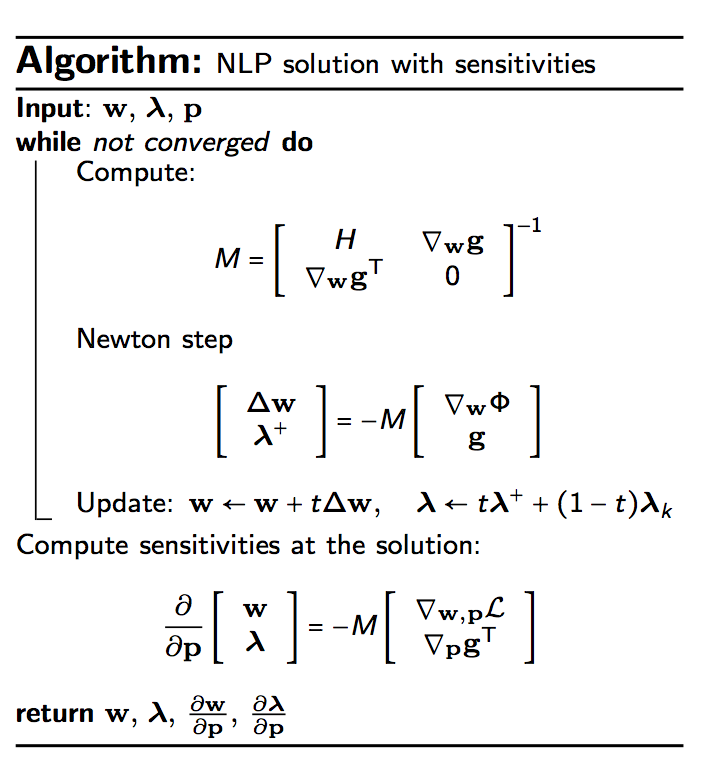
\includegraphics{NLP_newton}
				\end{figure}
	\end{itemize}
%%%%%%%%%%%%%%%%%%%%%%%%%%%%%%%%%%%%%%%%%%%%%%%%%%%%%%%%%%%%%%%%%%%%%%%
%%%%%%%%%%%%%%%%%%%%%%%%%%%%%%%%%%%%%%%%%%%%%%%%%%%%%%%%%%%%%%%%%%%%%%%
%%%%%%%%%%%%%%%%%%%%%%%%%%%%%%%%%%%%%%%%%%%%%%%%%%%%%%%%%%%%%%%%%%%%%%%
	\subsubsection{Sensitivity with inequality constraints}
		\begin{mini!}
			{w}{\Phi(w,p))}{}{}
			\addConstraint{g(w,p)=0}{}
			\addConstraint{h(w,p)\leq0}{}
		\end{mini!}	
	The solution $w(p),\lambda(p),\mu(p)$ is given by the KKT conditions:
	\begin{align*}
		\nabla_w\Lagrange(w,p,\lambda,\mu)&=0\\
		g(w,p)&=0\\
		h(w,p)\leq0\\
		\mu_ih_i(w,p)&=0
	\end{align*}
	Now we have non-smooth conditions; however, they are piecewise smooth.
	\par
	If we let $\mathbb{A}$ be the active set, then we have:
	\begin{align*}
		\nabla_w\Lagrange(w,p,\lambda,\mu)&=0\\
		g(w,p)&=0\\
		h_\mathbb{A}(w,p)&=0\\
		\mu_\mathbb{A}=0
	\end{align*}
	and $h_\mathbb{A}(w,p)<0,\mu_\mathbb{A}>0$. The conditions are smooth as long as all constraints are strictly active. Then we avoide the ``corner" of the complementarity slackness manifold.
	\par
	We know let $\mathbb{A}$ be the strictly active set and we have:
	\begin{align*}
		\nabla_w\Phi(w)+\nabla_wg(w,p)\lambda+\nabla_wh_\mathbb{A}(w,p)\mu_\mathbb{A}&=0\\
		g(w,p)&=0\\
		h_\mathbb{A}(w,p)&=0\\
		\mu_\mathbb{A}=0
	\end{align*}
	and $h_\mathbb{A}(w,p)<0,\mu_\mathbb{A}>0$. We then define
	\begin{align*}
		R(z,p)&=
		\begin{bmatrix}
			\nabla_w\Phi(w)+\nabla_wg(w,p)\lambda+\nabla_wh_\mathbb{A}(w,p)\mu_\mathbb{A}\\
			g(w,p)\\
			h_\mathbb{A}(w,p)
		\end{bmatrix}\\
		z&=
		\begin{bmatrix}
			w\\ \lambda \\ \mu_\mathbb{A}
		\end{bmatrix}
	\end{align*}
	The sensitivity is then given by $\frac{\partial z}{\partial p}=-\frac{\partial R(z,p)^{-1}}{\partial z}\frac{\partial R(z,p)}{\partial p}$ with :
	\begin{equation*}
		\frac{\partial R}{\partial z}=
		\begin{bmatrix}
			H & \nabla_wg & \nabla_wh_\mathbb{A}\\
			\nabla_wg^T & 0 & 0\\
			\nabla_wh_\mathbb{A}^T & 0 & 0
		\end{bmatrix}
	\end{equation*}
	The matrix $\frac{\partial R}{\partial z}$ is factorized inside Active Set QP solvers (i.e. we get the sensitivities for free when using SQP).
	\begin{exmp}
		\begin{mini!}
			{w}{\|w\|^2}{}{}
			\addConstraint{w_2-w_1(1+w_1^2)+\theta=0}{}
			\addConstraint{\frac{1}{5}(\tanh\theta+1)-w_2\leq0}{}
		\end{mini!}
		\begin{figure}[H]
			\centering
			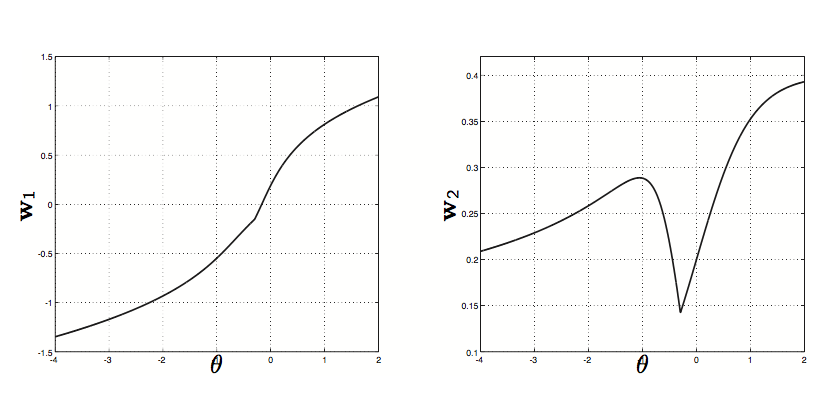
\includegraphics{NLP_example}
			\caption{}
		\end{figure}
		Writing the KKT conditions:
		\begin{align*}
			\frac{\partial}{\partial p}
			\begin{bmatrix}
				w\\ \lambda
			\end{bmatrix}\\
			&=-
			\begin{bmatrix}
				H & \nabla_wg\\
				\nabla_wg^T & 0
			\end{bmatrix}^{-1}
			\frac{\partial}{\partial p}
			\begin{bmatrix}
				\nabla_w\Lagrange\\
				g
			\end{bmatrix}\\
			\frac{\partial\mu}{\partial p}&=0
		\end{align*}
		Note that the constraint $h$ is inactive, $\mu=0$, $\mathbb{A}=\emptyset$.
		We then check $\frac{\partial z}{\partial \theta}$.
		\par
		At the ``corner" the derivative does not exist but the directional derivatives do, i.e. $\lim_{p\rightarrow p^-}\frac{\partial z}{\partial p}$ and $\lim_{p\rightarrow p^+}\frac{\partial z}{\partial p}$ exist.	
	\end{exmp}
%%%%%%%%%%%%%%%%%%%%%%%%%%%%%%%%%%%%%%%%%%%%%%%%%%%%%%%%%%%%%%%%%%%%%%%
%%%%%%%%%%%%%%%%%%%%%%%%%%%%%%%%%%%%%%%%%%%%%%%%%%%%%%%%%%%%%%%%%%%%%%%
	\subsection{Non-Smooth ``Linear" Approximator- QP approximation}
		\begin{mini!}
			{w}{\Phi(w,p)}{}{}
			\addConstraint{g(w,p)=0}{}
			\addConstraint{h(w,p)\leq0}{}
		\end{mini!}
		With the following sensitivities:
		\begin{equation*}
			\frac{\partial}{\partial p}
			\begin{bmatrix}
				w\\ \lambda \\ \mu
			\end{bmatrix}
			= -
			\begin{bmatrix}
				H & \nabla_wg & \nabla_wh\\
				\nabla_wg^T & 0 & 0\\
				\nabla_wh^T & 0 & 0
			\end{bmatrix}
			\frac{\partial}{\partial p}
			\begin{bmatrix}
				\nabla_w\Lagrange\\
				g\\
				h
			\end{bmatrix}
		\end{equation*}
		We can write the approximating QP:
		\begin{mini!}
			{\Delta w}{\frac{1}{2}\Delta w^TH\Delta w+\Delta p^T\nabla_{pw}\Lagrange\Delta w}{}{}
			\addConstraint{g+\nabla_wg^T\Delta g^T\Delta w+\nabla_pg^T\Delta p=0}{}
			\addConstraint{h+\nabla_wh^T\Delta h^T\Delta w+\nabla_ph^T\Delta p\leq0}{}
		\end{mini!}
		where $\Delta w= w-w_0$ and $\Delta p=p-p_0$.
		\par
		QP predictor holds the sensitivities implicitly (current active set) but also catches a linear approximation of the ``kinks" resulting from changes of active set.
%%%%%%%%%%%%%%%%%%%%%%%%%%%%%%%%%%%%%%%%%%%%%%%%%%%%%%%%%%%%%%%%%%%%%%%
%%%%%%%%%%%%%%%%%%%%%%%%%%%%%%%%%%%%%%%%%%%%%%%%%%%%%%%%%%%%%%%%%%%%%%%
%%%%%%%%%%%%%%%%%%%%%%%%%%%%%%%%%%%%%%%%%%%%%%%%%%%%%%%%%%%%%%%%%%%%%%%
	\subsubsection{Implementation}
	\begin{itemize}
		\item Solved at $p_0$ yields $w_0$
		\item New parameter $p$, perturbation $\Delta p=p-p_0$ inserted into the QP
		\item Predicted solution $w=w_0+\Delta w$ from the QP
	\end{itemize}
%%%%%%%%%%%%%%%%%%%%%%%%%%%%%%%%%%%%%%%%%%%%%%%%%%%%%%%%%%%%%%%%%%%%%%%
%%%%%%%%%%%%%%%%%%%%%%%%%%%%%%%%%%%%%%%%%%%%%%%%%%%%%%%%%%%%%%%%%%%%%%%
	\subsection{Off-line Path Following}
	Follow a solution path $w(p)$, for a given ``parameter trajectory" $p$. Below is the traditional SQP method using Newton steps.
	\begin{figure}[H]
		\centering
		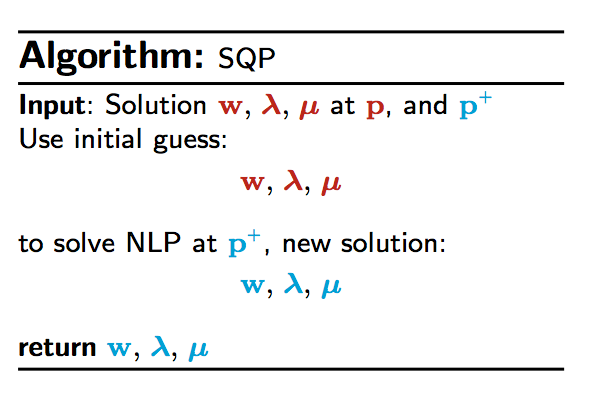
\includegraphics{NLP_SQP}
	\end{figure}
	The off-line path following SQP algorithm is outlined below.
	\begin{figure}[H]
		\centering
		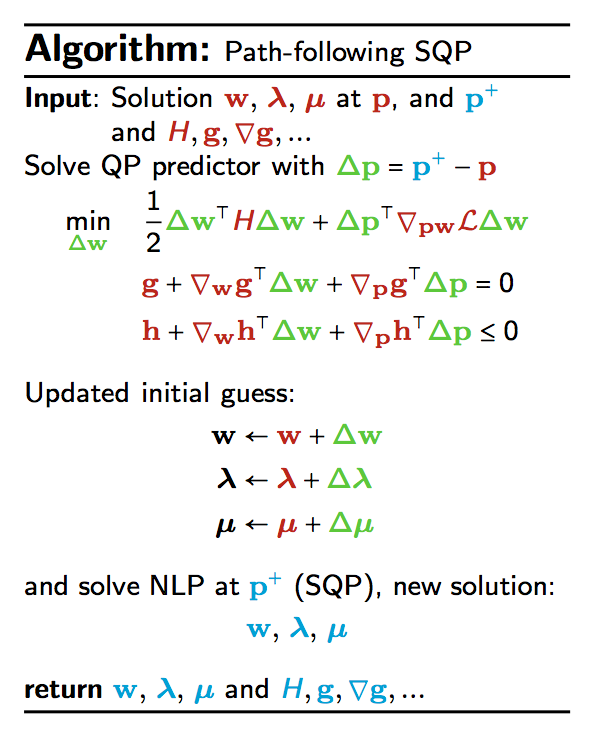
\includegraphics{SQP_path}
	\end{figure}
%%%%%%%%%%%%%%%%%%%%%%%%%%%%%%%%%%%%%%%%%%%%%%%%%%%%%%%%%%%%%%%%%%%%%%%
%%%%%%%%%%%%%%%%%%%%%%%%%%%%%%%%%%%%%%%%%%%%%%%%%%%%%%%%%%%%%%%%%%%%%%%
	\subsection{Predictor-Corrector}
	The QP predictor predicts solution for a parametric change in comparison to the SQP (corrector) which corrects the solution until KKT conditions are satisfied.
	\begin{mini!}
		{\Delta w}{\frac{1}{2}\Delta w^TH\Delta w +(p^+-p)^T\nabla_{pw}\Lagrange\Delta w}{}{}
		\addConstraint{g+\nabla_wg^T\Delta w+\nabla_pg^T(p^+-p)=0}{}
		\addConstraint{h+\nabla_wh^T\Delta w+\nabla_ph^T(p^+-p)=0}{}
	\end{mini!}
	The implementation is carried out as follows where the solution $w$ at $p$ is known, together with $H,g,\nabla g,\ldots$. For the new parameter $p^+$:
	\begin{itemize}
		\item Solve Predictor-Corrector, using $H,g,\nabla g,\ldots$ (already known). Predicts the next solution + correct $w$ if KKT not yet fulfilled
		\item Update $p\leftarrow p^+$, re-evaluate $H,g,\nabla g,\ldots,$ back to step 1. Correct solution until KKT satisfied.
	\end{itemize}
%%%%%%%%%%%%%%%%%%%%%%%%%%%%%%%%%%%%%%%%%%%%%%%%%%%%%%%%%%%%%%%%%%%%%%%
%%%%%%%%%%%%%%%%%%%%%%%%%%%%%%%%%%%%%%%%%%%%%%%%%%%%%%%%%%%%%%%%%%%%%%%
%%%%%%%%%%%%%%%%%%%%%%%%%%%%%%%%%%%%%%%%%%%%%%%%%%%%%%%%%%%%%%%%%%%%%%%
	\subsubsection{Predictor-Corrector and Parametric Embedding}
	NLP with parametric embedding is equivalent to the ``Path-following SQP" algorithm. This is a ``cheap" way of implementing the algorithm.
	The predictor-correct QP is as follows:
	\begin{mini!}
		{\Delta w,\Delta\theta}{\frac{1}{2}\Delta w^TH\Delta w +\nabla\Phi^T\Delta w+\Delta\theta^T\nabla_{\theta,w}\Lagrange\Delta w}{}{}
		\addConstraint{g+\nabla_wg^T\Delta w+\nabla_pg^T\Delta\theta=0}{}
		\addConstraint{h+\nabla_wh^T\Delta w+\nabla_ph^T\Delta\theta\leq0}{}
		\addConstraint{p-p^++\Delta\theta=0}{}
	\end{mini!}
	We note that if $p\neq p^+$, then the QP does a predictor-corrector step and sets $p\leftarrow p^+$ (full SQP step); if $p=p^+$, then QP does a classic SQP (corrector) step and converges to the KKT conditions.
%%%%%%%%%%%%%%%%%%%%%%%%%%%%%%%%%%%%%%%%%%%%%%%%%%%%%%%%%%%%%%%%%%%%%%%
%%%%%%%%%%%%%%%%%%%%%%%%%%%%%%%%%%%%%%%%%%%%%%%%%%%%%%%%%%%%%%%%%%%%%%%
	\subsection{Real-time Path Following: The real-time dilemma}
	Suppose that $p(t)$ is continuously changing with time $t$ and continuously measured. 
	In NMPC, $p(t)$ is a state estimation and the solution $w$ contains the control. We want to minimize time from $p(t)$ to update $w(p(t))$ (control delay).
	We also want to avoid linearization between the new $p(t)$ and the update of $w$.
	The algorithm for this method is outlined below.
	\begin{figure}[H]
		\centering
		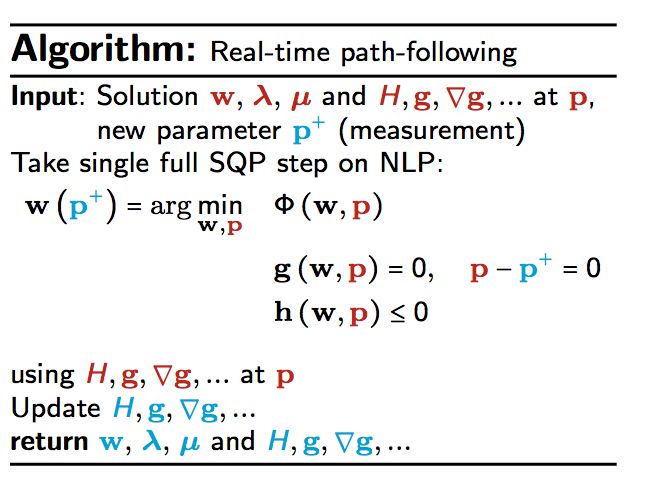
\includegraphics{real_time}
	\end{figure}
%%%%%%%%%%%%%%%%%%%%%%%%%%%%%%%%%%%%%%%%%%%%%%%%%%%%%%%%%%%%%%%%%%%%%%%
%%%%%%%%%%%%%%%%%%%%%%%%%%%%%%%%%%%%%%%%%%%%%%%%%%%%%%%%%%%%%%%%%%%%%%%
%%%%%%%%%%%%%%%%%%%%%%%%%%%%%%%%%%%%%%%%%%%%%%%%%%%%%%%%%%%%%%%%%%%%%%%
	\subsubsection{Real-Time Iteration (RTI) for NMPC}
	NMPC at physical time $i$ is an NLP with $w=\{x_0,u_0,\ldots,x_{N-1},u_{N-1},x_N\}$
	\begin{mini!}
		{w}{\Phi(w)}{}{}
		\addConstraint{g(w,\hat{x}_i)=\begin{bmatrix}\hat{x}_i-x_0\\f(x_0,u_0)-x_1\\ \ldots\\f(x_{N-1},u_{N-1})-x_N\end{bmatrix}}{}
		\addConstraint{h(w)=\begin{bmatrix}h(x_0,u_0)\\ \ldots\\h(x_{N-1},u_{N-1})\\h(x_N)\end{bmatrix}}{}
	\end{mini!}
	Note that the initial conditions $\hat{x}_i$ at time $i$ are already embedded in the formulation.
	We perform an initial preparation phase between $\hat{x}_{i-1}$ and $\hat{x}_i$:
	\begin{figure}[H]
		\centering
		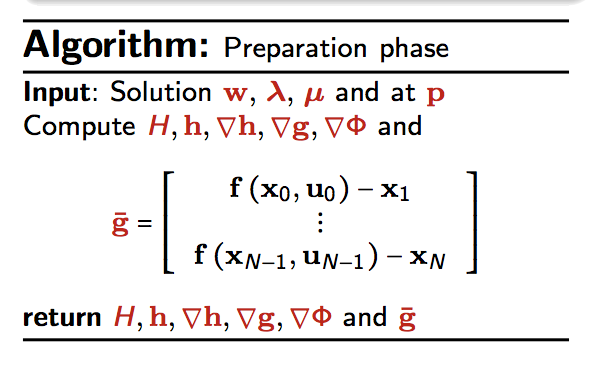
\includegraphics{prep_algo}
	\end{figure} 
	We then perform a feedback phase upon receiving $\hat{x}_i$:
	\begin{figure}[H]
		\centering
		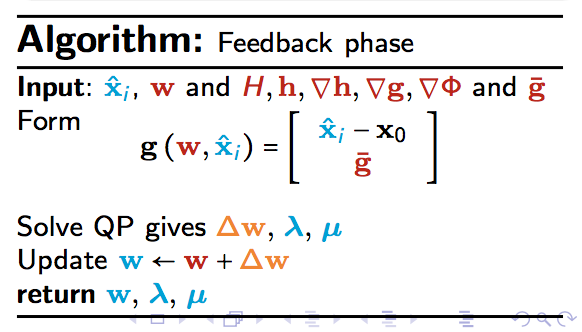
\includegraphics{feedback_algo}
	\end{figure}
	RTI reduces the control delay by moving the linearization ``out of the way" into the preparation phase. 
	The feedback phase becomes a simple QP problem to solve.
%%%%%%%%%%%%%%%%%%%%%%%%%%%%%%%%%%%%%%%%%%%%%%%%%%%%%%%%%%%%%%%%%%%%%%%
\section{Sensitivity-Based Economic NMPC with a Path-following Approach}
%%%%%%%%%%%%%%%%%%%%%%%%%%%%%%%%%%%%%%%%%%%%%%%%%%%%%%%%%%%%%%%%%%%%%%%
%%%%%%%%%%%%%%%%%%%%%%%%%%%%%%%%%%%%%%%%%%%%%%%%%%%%%%%%%%%%%%%%%%%%%%%
\subsection{Introduction}
	The idea of economic model predictive control (MPC) is to integrate the economic optimization layer and the control layer in the process control hierarchy into a single dynamic optimization layer.
	Economic MPC adjusts the inputs to minimize the economic cost of operation directly.
	\par
	Since nonlinear process models are often used for economic optimization, a potential drawback of economic MPC is that it requires solving a large-scale nonlinear optimization problem (NLP) associated with the nonlinear model predictive control (NMPC) problem at every sample time.
	The solution of this NLP may take a significant amount of time and this can lead to performance degradation and even to instability of the closed-loop system.
	\par
	Instead of solving the full nonlinear optimization problem when new measurements of the state become available, these approaches use the sensitivity of the NLP solution at a previously-computed iteration to obtain fast approximate solutions to the new NMPC problem.
	These can be implemented in the plant with minimal delay.
	\par
	The concept of real-time iteration (RTI), in which the full NLP is not solved at all during the MPC iterations.
	Instead, at each NMPC sampling time, a single quadratic programming (QP) related to the sequential quadratic programming (SQP) iteration for solving the full NLP is solved.
	The real-time iteration scheme contains two phases: (1) the preparation phase and (2) the feedback phase.
	In the preparation phase, the model derivatives are evaluated using a predicted state measurement, and a QP is formulated based on data of this predicted state.
	In the feedback phase, once the new initial state is available, the QP is updated to include the new initial state and solved for the control input that is injected into the plant.
	\par
	A different approach known as advanced-step NMPC (asNMPC) involves solving the full NLP at each sample time.
	However, the full NLP solution is computed in advance for a predicted initial state.
	Once the new state measurement is available, the NLP solution is corrected using a fast sensitivity update to match the measured or estimated initial state.
	\par
	In this case, we apply an improved path-following method for correcting the NLP solution within the advanced-step NMPC framework.
	We use asNMPC with a predictor-corrector path-following algorithm that is able to perform even in the presence of measurement noise.
%%%%%%%%%%%%%%%%%%%%%%%%%%%%%%%%%%%%%%%%%%%%%%%%%%%%%%%%%%%%%%%%%%%%%%%
%%%%%%%%%%%%%%%%%%%%%%%%%%%%%%%%%%%%%%%%%%%%%%%%%%%%%%%%%%%%%%%%%%%%%%%
\subsection{NMPC Problem Formulations}
%%%%%%%%%%%%%%%%%%%%%%%%%%%%%%%%%%%%%%%%%%%%%%%%%%%%%%%%%%%%%%%%%%%%%%%
%%%%%%%%%%%%%%%%%%%%%%%%%%%%%%%%%%%%%%%%%%%%%%%%%%%%%%%%%%%%%%%%%%%%%%%
%%%%%%%%%%%%%%%%%%%%%%%%%%%%%%%%%%%%%%%%%%%%%%%%%%%%%%%%%%%%%%%%%%%%%%%
\subsubsection{The NMPC Problem}
We consider a nonlinear discrete-time dynamic system:
\begin{equation*}
	x_{k+1} = f(x_k,u_k)
\end{equation*}
where $x_k\in\mathbb{R}^{n_x}$ denotes the state variable, $u_k\in\mathbb{R}^{n_u}$ is the control input and $f:\mathbb{R}^{n_x}\times\mathbb{R}^{n_u}\rightarrow R^{n_x}$ is a continuous model function, which calculates the next state $x_{k+1}$ from the previous state $x_k$ and control input $u_k$, where $k\in\mathbb{N}$.
This system is optimized by a nonlinear model predictive controller, which solves the problem:
	\begin{mini!}
		{z_l,v_l}{\Psi(z_N)+\sum_{l=0}^{N-1}\psi(z_l,v_l)}{}{}
		\addConstraint{z_{i+1}=f(z_l,v_l)}{l=0,\ldots,N-1}
		\addConstraint{z_0=x_k}{}
		\addConstraint{(z_l,v_l)\in\mathcal{Z},}{l=0,\ldots,N-1}
		\addConstraint{z_N\in X_f}{}
		\label{eq:NMPC}
	\end{mini!}
at each sample time.
Here, $z_i\in\mathbb{R}^{n_x}$ is the predicted state variable; $v_l\in\mathbb{R}^{n_u}$ is the predicted control input; and $z_N\in\mathcal{X}_f$ is the final predicted state variable restricted to the terminal region $\mathcal{X}_f\in\mathbb{R}^{n_x}$.
The stage cost is denoted by $\psi:\mathbb{R}^{n_x}\times\mathbb{R}^{n_u}\rightarrow\mathbb{R}$ and the terminal cost by $\Psi:\mathcal{X}_f\rightarrow\mathbb{R}$.
Further $\mathcal{Z}$ denotes the path constraints, i.e. $\mathcal{Z}=\{(z,v)|q(z,v)\leq0\}$, where $q:\mathbb{R}^{n_x}\times\mathbb{R}^{n_u}\leftarrow\mathbb{R}^{n_q}$.
\par
The solution of the optimization problem is denoted $\{z_0^*,\ldots,z_N^*,v_0^*,\ldots,v_{N-1}^*\}$.
At sample time $k$, an estimate or measurement of the state $x_k$ is obtained and the problem shown above (\ref{eq:NMPC}) is solved.
Then, the first part of the optimal control sequence is assigned as plant input such that $u_k=v_0^*$.
The first part of the solution defines an implicit feedback law and the system will evolve according to $x_{k+1}=fr(x_k,\kappa(x_k))$.
At the next sample time $k+1$, when the measurement of the new state $x_{k+1}$ is obtained, the procedure is repeated.
The NMPC algorithm is summarized below.
\begin{figure}[H]
	\centering
	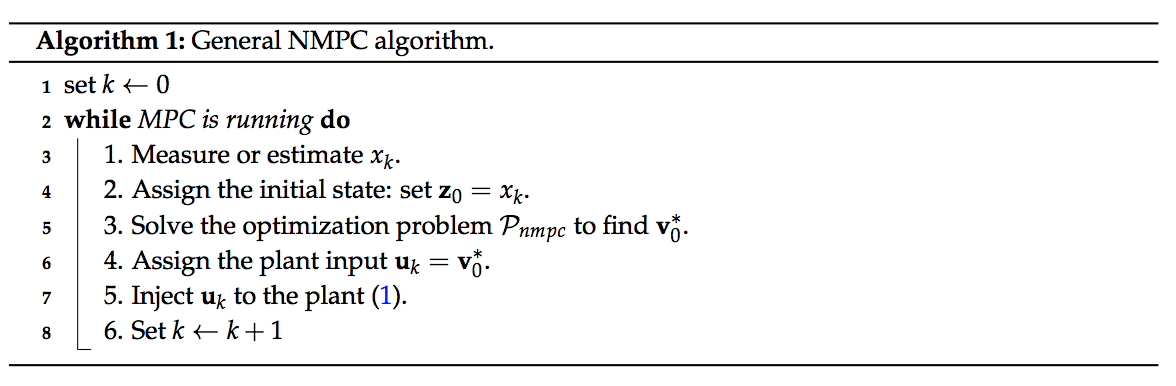
\includegraphics{NMPC_algo}
\end{figure}
%%%%%%%%%%%%%%%%%%%%%%%%%%%%%%%%%%%%%%%%%%%%%%%%%%%%%%%%%%%%%%%%%%%%%%%
%%%%%%%%%%%%%%%%%%%%%%%%%%%%%%%%%%%%%%%%%%%%%%%%%%%%%%%%%%%%%%%%%%%%%%%
%%%%%%%%%%%%%%%%%%%%%%%%%%%%%%%%%%%%%%%%%%%%%%%%%%%%%%%%%%%%%%%%%%%%%%%
\subsubsection{Ideal NMPC and Advanced-Step NMPC Framework}
	We refer to the hypothetical case where the NMPC problem can be solved instantaneously as ideal NMPC.
	In practice, there will be of course some time delay between obtaining the updated values of the states and injecting the updated inputs into the plant.
	The main reason for this delay is the time it requires to solve the optimization problem.
	\par
	This has lead to the development of fast senstivity-based NMPC approaches.
	We will now look at the advanced-step NMPC (asNMPC) approach, which is based on the following steps:
	\begin{enumerate}[label=(\alph*)]
		\item Solve the NMPC problem at time $k$ with a predicted state value of time $k+1$ 
		\item When the measurement $x_{k+1}$ becomes available at time $k+1$, compute an approximation of the NLP solution using fast sensitivity methods
		\item Update $k\leftarrow k+1$ and repeat from Step 1
	\end{enumerate}
	\par
	It has been proposed that a fast one-step sensitivity update that is based on solving a linear system of equations.
	Under some assumptions, this corresponds to a first-order Taylor approximation of the optimal solution.
	In particular, this approach requires strict complementarity of the NLP solution, which ensures no changes in the active set.
	A more general approach involves allowing for changes in the active set and making several sensitivity updates.
	This approach will be focused on here.
%%%%%%%%%%%%%%%%%%%%%%%%%%%%%%%%%%%%%%%%%%%%%%%%%%%%%%%%%%%%%%%%%%%%%%%
%%%%%%%%%%%%%%%%%%%%%%%%%%%%%%%%%%%%%%%%%%%%%%%%%%%%%%%%%%%%%%%%%%%%%%%
\subsection{Sensitivity-Based Path-Following NMPC}
%%%%%%%%%%%%%%%%%%%%%%%%%%%%%%%%%%%%%%%%%%%%%%%%%%%%%%%%%%%%%%%%%%%%%%%
%%%%%%%%%%%%%%%%%%%%%%%%%%%%%%%%%%%%%%%%%%%%%%%%%%%%%%%%%%%%%%%%%%%%%%%
%%%%%%%%%%%%%%%%%%%%%%%%%%%%%%%%%%%%%%%%%%%%%%%%%%%%%%%%%%%%%%%%%%%%%%%
\subsubsection{Sensitivity Properties of NLP}
The dynamic optimization problem shown in Problem (\ref{eq:NMPC}) can be cast as a general parametric NLP problem.
	\begin{mini!}
		{\chi}{F(\chi,p)}{}{}
		\addConstraint{c(\chi,p)=}{0}
		\addConstraint{g(\chi,p)\leq}{0}
		\label{eq:NLP}
	\end{mini!}
	where $\chi\in\mathbb{R}^{n_\chi}$ are the decision variables (typically the state variables and the control input) and $p\in\mathbb{R}^{n_p}$ is the parameter, which is typically the initial state variable $x_k$.
	In addition $F:\mathbb{R}^{n_\chi}\times\mathbb{R}^{n_p}\rightarrow\mathbb{R}$ is the scalar objective function; $c:\mathbb{R}^{n_\chi}\times\mathbb{R}^{n_p}\rightarrow\mathbb{R}^{n_c}$ denotes the equality constraints; and finally, $g:\mathbb{R}^{n_\chi}\times\mathbb{R}^{n_p}\rightarrow\mathbb{R}^{n_g}$ denotes the inequality constraints.
	The instances in Problem (\ref{eq:NLP}) that are solved at each sample time differ only in the parameter $p$.
	\par
	The Lagrangian of this problem is:
	\begin{equation}
		\Lagrange(\chi,p,\lambda,\mu)=F(\chi,p)+\lambda^Tc(\chi,p)+\mu^Tg(\chi,p)
	\end{equation}
	and the KKT conditions are:
	\begin{align}
		c(x,p)&=0,\qquad g(x,p)\leq 0 \qquad \text{ (primal feasibility) }\label{eq:primal}\\
		\mu&\geq0, \qquad \text{ (dual feasibility) }\nonumber\\
		\nabla_x\Lagrange(x,p,\lambda,\mu)&=0, \qquad \text{ (stationary condition) }\nonumber\\
		\mu^Tg(x,p)&=0, \qquad \text{ (complementary slackness) }\nonumber
	\end{align}
	\par
	In order for the KKT conditions to be a necessary condition of optimality, we require a constraint qualification (CQ) to hold.
	From now on we assume that the linear independence constraint qualification (LICQ) holds:
	\begin{definition}[LICQ]
		\textit{Given a vector $p$ and a point $\chi$, the LICQ holds at $\chi$ if the set of vectors $\{\{\nabla_\chi c_i(\chi,p)\}_{i\in\{1,\ldots,n_c\}}\cup\{\nabla_{\chi}g_i(\chi,p)\}_{i:g_i(\chi,p)=0}\}$ is linearly independent.}
	\end{definition}
	\par
	The LICQ implies that the multipliers $(\lambda,\mu)$ satisfying the KKT conditions are unique.
	If additionally, a suitable second-order condition holds, then the KKT conditions guarantee a unique local minimum.
	A suitable second-order condition states that the Hessian matrix has to be positive definite in a set of appropriate directions, defined by the following property:
	\begin{definition}[SSOSC]
		\textit{The strong second-order sufficient condition (SSOSC) holds at $\chi$ with multipliers $\lambda$ and $\mu$ if $d^T\nabla_\chi^2\Lagrange(\chi,p,\lambda,\mu)d>0$ for all $d\neq0$, such that $\nabla_\chi c(\chi,p)^Td=0$ and $\nabla_\chi g_i(\chi,p)^Td=0$ for $i$ such that $g_i(\chi,p)=0$ and $\mu_i>0$.
		}
	\end{definition}
	\par
	For a given $p$, we denote the solution to (\ref{eq:NLP}) by $\chi^*(p),\lambda^*(p),\mu^*(p)$, and if possible, we omit the argument.
	We want to know how the solution changes with a perturbation in the parameter $p$.
	One more important concept is outlined below:
	\begin{definition}[SC]
		Given a vector $p$ and a solution $\chi^*$ with vectors of multipliers $\lambda^*$ and $\mu^*$, strict complimentary (SC) holds if $\mu_i^*-g_i(\chi^*,p)>0$ for each $i=1,\ldots,n_g$.
	\end{definition}
	We now look at the result.
	\begin{theorem}[Implicit function theorem applied to optimality conditions]
		Let $\chi^*(p)$ be a KKT point that satisfies (\ref{eq:primal}), and assume that LICQ, SSOSC, and SC hold at $\chi^*$.
		Further, let the function $F,c,g$ be at least $k+1$ times differentiable in $\chi$ and $k$-times differentiable in $p$. Then:
		\begin{itemize}
			\item $\chi^*$ is an isolated minimizer, and the associated multipliers $\lambda$ and $\mu$ are unique.
			\item for $p$ in a neighborhood of $p_0$, the set of active constraints remains unchanged
			\item for $p$ in a neighborhood of $p_0$, there exists a $k-times$ differentiable function $\sigma(p)=\begin{bmatrix}\chi^*(p)^T &\lambda^*(p)^T & \mu^*(p)^T\end{bmatrix}$, that corresponds to a locally unique minimum for (\ref{eq:primal}).
		\end{itemize}
	\end{theorem}
	\par
	Using this result, the sensitvity of the optimal solution $\chi^*,\lambda^*,\mu^*$ in a small neighborhood of $p_0$ can be computed by solving a system of linear equations that arises from applying the implicit function theorem to the KKT conditions:
	\begin{equation}
		\begin{bmatrix}
			\nabla_{\chi\chi}^2\Lagrange(\chi^*,p_0,\lambda^*,\mu^*)&\nabla_\chi c(\chi^*,p_0)&\nabla_\chi g_A(\chi^*,p_0)\\
			\nabla_\chi c(\chi^*,p_0)^T & 0 & 0\\
			\nabla_\chi g_A(\chi^*,p_0)^T & 0 & 0
		\end{bmatrix}
		\begin{bmatrix}
			\nabla_p\chi\\
			\nabla_p\lambda\\
			\nabla_p\mu
		\end{bmatrix}
		=-
		\begin{bmatrix}
			\nabla_{p\chi}^2\Lagrange(\chi^*,p_0,\lambda^*,\mu^*)\\
			\nabla_p c(\chi^*,p_0)\\
			\nabla_p g_A(\chi^*,p_0)
		\end{bmatrix}
		\label{eq:NLP_KKT}
	\end{equation}
	\par
	Here, the constraint gradients with subscript $g_A$ indicate that we only include the vectors and components of the Jacobian corresponding to the active inequality constraints at $\chi$, i.e., $i\in A$ if $g_i(\chi,p_0)=0$.
	Denoting the solution of the equation above as $\begin{bmatrix}\nabla_p\chi & \nabla_p\lambda & \nabla_p\mu\end{bmatrix}^T$, for small $\Delta p$, we obtain a good estimate:
	\begin{align}
		\chi(p_0+\Delta p)&=\chi^*+\nabla_p\chi\Delta p\\
		\lambda(p_0+\Delta p)&=\lambda^*+\nabla_p\lambda\Delta p\\
		\mu(p_0+\Delta p)&=\mu^*+\nabla_p\mu\Delta p
	\end{align}
	of the solution to the NLP Problem (\ref{eq:NLP}) at the parameter value $p_0+\Delta p$.
	\par
	If $\Delta p$ becomes large, the approximate solution may no longer be accurate enough because the SC assumption implies that the active set cannot change. 
	While this is true for small perturbations, large changes in $\Delta p$ may very well induce active set changes.
	\par
	It can be seen that the sensitivity system corresponds to the stationary conditions for a particular QP.
	If $\Delta p$ is small enough, we can show that the set $\{i:\mu(\bar{p})_i>0\}$ is constant for $\bar{p}=p_0+\Delta p$.
	Thus we can form a QP wherein we are potentially moving off of weakly-active constraints while staying on the strongly-active ones.
	The primal-dual solution of this QP is in fact the directional derivative of the primal-dual solution $\chi^*(p),\lambda^*(p),\mu^*(p)$.
	\begin{theorem}
		Let $F,c,g$ be twice continuously differentiable in $p$ and $\chi$ near $(\chi^*,p_0)$ and let the LICQ and SSOSC hold at $(\chi^*,p_0)$.
		Then, the solution $(\chi^*(p),\lambda^*(p),\mu^*(p))$ is Lipschitz continuous in a neighborhood of $(\chi^*,\lambda^*,\mu^*,p_0)$ and the solution function $(\chi^*(p),\lambda^*(p),\mu^*(p))$ is directionally differentiable.
		\par
		Moreover, the directional derivative uniquely solves the following quadratic problem:
		\begin{mini!}
			{\Delta\chi}{\frac{1}{2}\Delta\chi^T\nabla_{\chi\chi}^2\Lagrange(\chi^*,p_0,\lambda^*,\mu^*)\Delta\chi+\Delta\chi^T\nabla_{p\chi}^2\Lagrange(\chi^*,p_0,\lambda^*,\mu^*)\Delta p}{}{}
			\addConstraint{\nabla_\chi c_i(\chi^*,p_0)^T\Delta\chi+\nabla_p c_i(\chi^*,p_0)^T\Delta p}{=0,\qquad i=1,\ldots,n_c}
			\addConstraint{\nabla_\chi g_j(\chi^*,p_0)^T\Delta\chi+\nabla_p g_j(\chi^*,p_0)^T\Delta p}{=0,\qquad j\in K_+}
			\addConstraint{\nabla_\chi g_j(\chi^*,p_0)^T\Delta\chi+\nabla_p g_j(\chi^*,p_0)^T\Delta p}{\leq 0, \qquad j\in K_0}
			\label{eq:QP_pred}
		\end{mini!}
	where $K_+=\{j\in\mathbb{Z}:\mu_j>0\}$ is the strongly-active set and $K_0=\{j\in\mathbb{Z}:\mu_j=0 \text{ and } g_j(\chi^*,p_0)=0\}$ denotes the weakly active set.
	\end{theorem}
	\par
	The theorem above gives the solution of the perturbed NLP by solving a QP problem.
	Note that as the solution to this QP is the directional derivative of the primal-dual solution of the NLP, it is a predictor step, a tangential first-order estimate of the change in the solution subject to a change in the parameter.
	We refer to the QP (\ref{eq:QP_pred}) as a pure-predictor.
	Note that obtaining the sensitivity via this method has the advantage that changes in the active set can be accounted for correctly and strict complementarity (SC) is not required.
%%%%%%%%%%%%%%%%%%%%%%%%%%%%%%%%%%%%%%%%%%%%%%%%%%%%%%%%%%%%%%%%%%%%%%%
%%%%%%%%%%%%%%%%%%%%%%%%%%%%%%%%%%%%%%%%%%%%%%%%%%%%%%%%%%%%%%%%%%%%%%%
%%%%%%%%%%%%%%%%%%%%%%%%%%%%%%%%%%%%%%%%%%%%%%%%%%%%%%%%%%%%%%%%%%%%%%%
\subsubsection{Path-Following Based on Sensitivity Properties}
Equation \ref{eq:NLP_KKT} and the QP (\ref{eq:QP_pred}) describes the change in the optimal solutions for small perturbations.
They are not guaranteed to reproduce the optimal solution accurately for larger perturbations.
One approach to handle such cases is to divide the overall perturbation into several smaller intervals and to iteratively use the sensitivity to track the path of optimal solutions.
\par
The general idea of a path-following method is to reach the solution of the problem at a final parameter value $p_f$ by tracing a sequence of solutions $(\chi_k,\lambda_k,\mu_k)$ for a series of parameter values $p(t_k)=(1-t_k)p_0+t_kp_f$ with $0=t_0<t_1<\ldots<t_k<\ldots<t_N=1$.
The new direction is found by evaluating the sensitivity at the current point (i.e. similar Euler integration for ODE).
\par
A path-following algorithm that is only based on the sensitivity calculated by the pure predictor QP may fail to track the solution accurately enough and may lead to poor solutions.
A common approach to address this problem is to include elements that are similar to a Newton step, which force the path-following algorithm towards the true solution.
If we approximate (\ref{eq:NLP})by a QP, linearizing with respect to both $\chi$ and $p$, and enforce the equality of the strongly-active constraints:
	\begin{mini!}
		{\Delta\chi\Delta p}{\scriptstyle\frac{1}{2}\Delta_{\chi\chi}^2\Lagrange(\chi^*,p_0,\lambda^*,\mu^*)\Delta\chi+\Delta\chi^T\nabla_{p\chi}^2\Lagrange(\chi^*,p_0,\lambda^*,\mu^*)\Delta p+\nabla_\chi F^T\Delta\chi+\nabla_p F\Delta p+\frac{1}{2}\Delta p^T\nabla_{pp}^2\Lagrange(\chi^*,p_0,\lambda^*,\mu^*)\Delta p}{}{}
		\addConstraint{c_i(\chi^*,p_0)+\nabla_\chi c_i(\chi^*,p_0)^T\Delta\chi+\nabla_p c_i(\chi^*,p_0)^T\Delta p=0}{\qquad i=0,\ldots,n_c}
		\addConstraint{g_j(\chi^*,p_0)+\nabla_\chi g_j(\chi^*,p_0)^T\Delta\chi+\nabla_p g_j(\chi^*,p_0)^T\Delta p=0}{\qquad j\in K_+}
		\addConstraint{g_j(\chi^*,p_0)+\nabla_\chi g_j(\chi^*,p_0)^T\Delta\chi+\nabla_p g_j(\chi^*,p_0)^T\Delta p\leq0}{\qquad j\in\{1,\ldots,n_g\}/K_+}
	\end{mini!}
	\par
	In the NMPC problem, the parameter $p$ corresponds to the current ``initial" state $x_k$.
	Moreover, the cost function is independent of $p$ and we have that $\nabla_pF=0$.
	We then get that $\nabla_pc$ and $\nabla_pg$ are constants.
	Thus the above QP formulation can simplify to:
		\begin{mini!}
		{\Delta\chi\Delta p}{\frac{1}{2}\Delta_{\chi\chi}^2\Lagrange(\chi^*,p_0,\lambda^*,\mu^*)\Delta\chi+\nabla_\chi F^T\Delta\chi}{}{}
		\addConstraint{c_i(\chi^*,p_0)+\nabla_\chi c_i(\chi^*,p_0)^T\Delta\chi=0}{\qquad i=0,\ldots,n_c}
		\addConstraint{g_j(\chi^*,p_0)+\nabla_\chi g_j(\chi^*,p_0)^T\Delta\chi=0}{\qquad j\in K_+}
		\addConstraint{g_j(\chi^*,p_0)+\nabla_\chi g_j(\chi^*,p_0)^T\Delta\chi\leq0}{\qquad j\in\{1,\ldots,n_g\}/K_+}
		\label{eq:QP_predcorr}
	\end{mini!}
	\par
	We denote the QP formulation (\ref{eq:QP_predcorr}) as the predictor-corrector.
	While this appears similar to the QP proposed in the real-time iteration scheme, we note that it differs because here we enforce the strongly-active constraints as as equality constraints in the QP.
	\par
	The predictor-corrector QP (\ref{eq:QP_predcorr}) is well suited for use in a path-following algorithm, where the optimal solution path is tracked from $p_0$ to a final value $p_f$ along a sequence of parameter points $p(t_k)=(1-t_k)p_0+t_kp_f$ with $0=t_0<t_1<\ldots<t_k<\ldots<t_N=1$.
	At each point $p(t_k)$, the QP is solved and the primal-dual solutions updated as:
	\begin{align}
		\chi(t_{k+1})&=\chi(t_k)+\Delta\chi\\
		\lambda(t_{k+1})&=\Delta\lambda\\
		\mu(t_{k+1})&=\Delta\mu
	\end{align}
where $\Delta\chi$ is obtained from the primal solution of QP (\ref{eq:QP_predcorr}) and where $\Delta\lambda$ and $\Delta\mu$ correspond to the Lagrange multipliers of QP (\ref{eq:QP_predcorr}).
	\par
	Changes in the active set along the path are detected by the QP as follows: If a constraint becomes inactive at some point along the path, the corresponding multiplier $\mu_j$ will first become weakly active, i.e, it will be added to the set $K_0$.
	Since this is not included as an equality constraint, the next QP solution could move away from the constraint.
	Similarly, if a new constraint $g_j$ becomes active along the path, it will make the corresponding linearized inequality constraint in the QP active.
	\par
	The resulting path-following algorithm is summarized with its main steps in Algorithm 2.
	\begin{figure}[H]
		\centering
		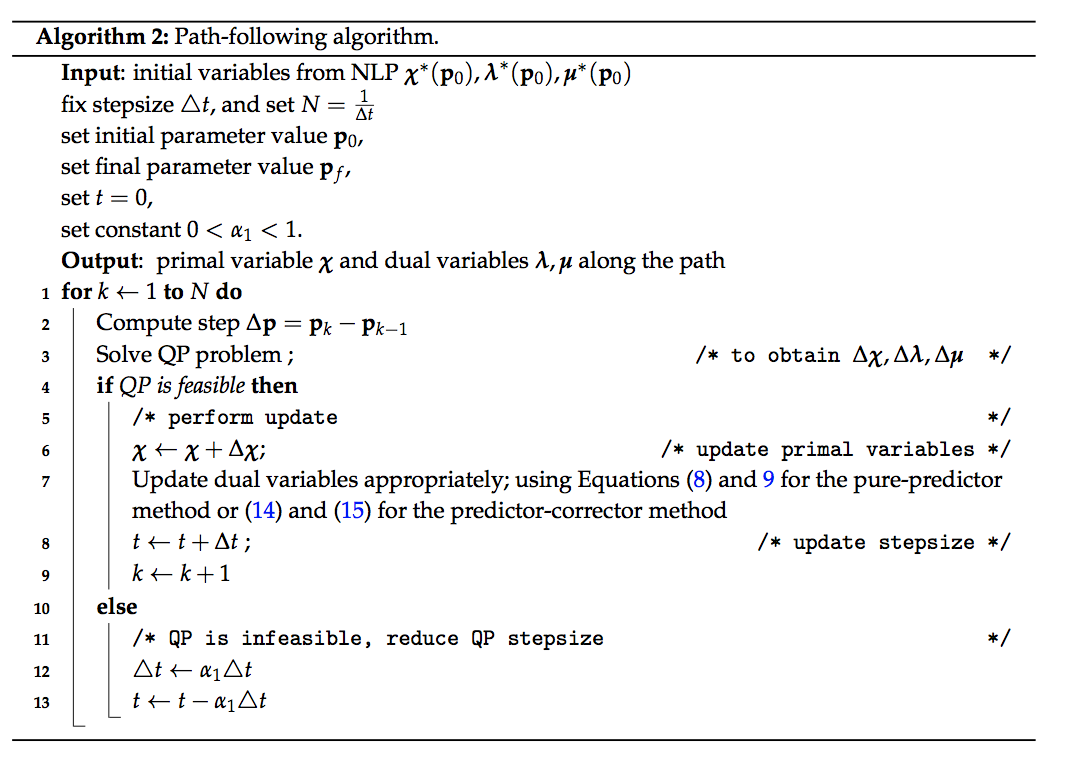
\includegraphics[scale=0.6]{pred_corr_algo}
		%\caption{}
	\end{figure}
%%%%%%%%%%%%%%%%%%%%%%%%%%%%%%%%%%%%%%%%%%%%%%%%%%%%%%%%%%%%%%%%%%%%%%%
%%%%%%%%%%%%%%%%%%%%%%%%%%%%%%%%%%%%%%%%%%%%%%%%%%%%%%%%%%%%%%%%%%%%%%%
%%%%%%%%%%%%%%%%%%%%%%%%%%%%%%%%%%%%%%%%%%%%%%%%%%%%%%%%%%%%%%%%%%%%%%%
\subsubsection{Discussion of the Path-Following asNMPC Approach}
We now concentrate on the advanced-step NMPC framework, i.e., at every time step, the full NLP is solved for a predicted state.
When the new measurement becomes available, the precomputed NLP solution is updated by tracking the optimal solution curve from the predicted initial state to the new measured or estimated state.
Note that any numerical homotopy algorithm can be used to update the NLP solution.
The solution of the last QP along the path corresponds to the updated NLP solution and only the inputs computed in this last QP will be injected into the plant.
\par
This situation differs from the RTI scheme previously described where the NLP is not solved at all during the MPC sampling times.
Instead, at each sampling time, a single QP is solved and the computed input is applied to the palnt.
This requires rapid sampling times, and if the QP fails to track the true solution then other measures have to be performed to get the controller ``on-track" again.
\par
In comparison to previously published studies, strongly- and weakly- active inequality constraints are distinguished.
Strongly-active inequalities are included as linearized equality contraints in the QP and weakly-active constraints are linearized and added as inequality constraints to the QP.
This helps ensure that the true solution path is tracked more accurately when dealing with a non-convex full Hessian.
%%%%%%%%%%%%%%%%%%%%%%%%%%%%%%%%%%%%%%%%%%%%%%%%%%%%%%%%%%%%%%%%%%%%%%%
%%%%%%%%%%%%%%%%%%%%%%%%%%%%%%%%%%%%%%%%%%%%%%%%%%%%%%%%%%%%%%%%%%%%%%%
\subsection{Numerical Case Study}
%%%%%%%%%%%%%%%%%%%%%%%%%%%%%%%%%%%%%%%%%%%%%%%%%%%%%%%%%%%%%%%%%%%%%%%
%%%%%%%%%%%%%%%%%%%%%%%%%%%%%%%%%%%%%%%%%%%%%%%%%%%%%%%%%%%%%%%%%%%%%%%
%%%%%%%%%%%%%%%%%%%%%%%%%%%%%%%%%%%%%%%%%%%%%%%%%%%%%%%%%%%%%%%%%%%%%%%
\subsubsection{Process Description}
	We now look at the path-following NMPC (pf-NMPC) on an isothermal reactor and separator process depicted in Figure \ref{fig:reactor}.
The CSTR is fed with a stream $F_0$ containing 100\% component $\mathcal{A}$ and a recycler $R$ from the distillation column.
A first-order reaction \ce{A -> B} takes place in the CSTR where $\mathcal{B}$ is the desired product and the product with flow rate $F$ is fed to the column.
In the distillation column, the unreacted raw material is separated from the product and recycled back to the reactor.
The desired product $\mathcal{B}$ leaves the distillation column as the bottom product, which has a purity requirement.
The model for the process has 84 state variables of which 82 of which are from the distillation and two from the CSTR.
	\begin{figure}[H]
		\centering
		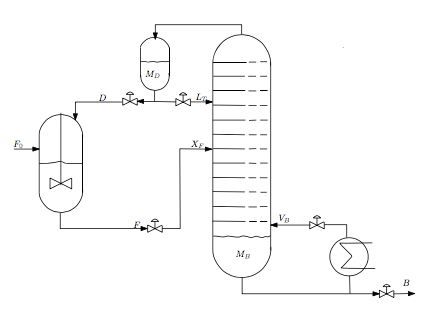
\includegraphics{reactor}
		\caption{CSTR and distillation column}
		\label{fig:reactor}
	\end{figure}
\par
The stage cost of the economic objective function to optimize under operation is:
\begin{equation}
	J=p_FF_0+p_VV_B-p_BB
\end{equation}
where $p_F$ is the feed cost $p_V$ is the steam cost and $p_B$ is the product price.
The operational constraints are the concentration of the bottom product as well as the liquid holdup at the bottom and top of the distillation column and in the CSTR.
The control inputs are the reflux flow ($L_T$), boil-up flow ($V_B$), feeding rate to the distillation ($F$), distillate (top) and bottom product flow rates ($D$ and $B$).
\par
First we ran a steady-state optimization with a feed rate of $F_0=0.3$(\si{\kilo\mole\per\minute}).
This gives us the optimal values for control inputs and state variables; the optimal steady state input values are $u_s=\begin{bmatrix} 1.18 & 1.92&1.03&0.74&0.29\end{bmatrix}^T$.
These values are used to construct the regularization term added to the objective function.
We thus end up with the regularized stage:
\begin{equation}
	J_m=p_FF_0+p_VV_B-p_BB-p_DD+(z-x_s)^TQ_1(z-x_s)+(v-u_s)^TQ_2(v-u_s)
\end{equation}
The weights $Q_1$ and $Q_2$ are selected to make the rotated stage cost of the steady state problem strongly convex; this ensures that the NMPC controller is stable.
\par
We then set up the NLP for calculating the predicted state variables $z$ and predicted control inputs $v$.
We use direct collocation on finite elements using Lagrange collocation to discretize the dynamics, using three colocation points in each finite element.
This allows the state variables and control inputs to become optimization variables.
\par
The economic NMPC case study is simulated with 150 MPC iterations with a sample time of 1 min.
The prediction horizon is set to 30 min.
These settings result in an NLP with 10,314 optimization variables.
CasADi and IPOPT are used as the NLP solver.
The QPs are solved using MINOS QP from TOMLAB.
%%%%%%%%%%%%%%%%%%%%%%%%%%%%%%%%%%%%%%%%%%%%%%%%%%%%%%%%%%%%%%%%%%%%%%%
%%%%%%%%%%%%%%%%%%%%%%%%%%%%%%%%%%%%%%%%%%%%%%%%%%%%%%%%%%%%%%%%%%%%%%%
%%%%%%%%%%%%%%%%%%%%%%%%%%%%%%%%%%%%%%%%%%%%%%%%%%%%%%%%%%%%%%%%%%%%%%%
\subsubsection{Open-Loop Results}
We observe that the one-step pure-predictor tracks the ideal NMPC solution the worst and the four-step path-following with predictor-corrector tracks best.
This is due to the fact that the predictor-correct path-following QP has an additional linear term in the objective function and constraint for the purpose of moving closer to the solution of the NLP, as well as tracing the first-order estimate of the change in the solution.
\par
In this case study, we note that a single predictor-corrector step has almost as good performance as the four predictor-corrector steps along the path.
%%%%%%%%%%%%%%%%%%%%%%%%%%%%%%%%%%%%%%%%%%%%%%%%%%%%%%%%%%%%%%%%%%%%%%%
%%%%%%%%%%%%%%%%%%%%%%%%%%%%%%%%%%%%%%%%%%%%%%%%%%%%%%%%%%%%%%%%%%%%%%%
%%%%%%%%%%%%%%%%%%%%%%%%%%%%%%%%%%%%%%%%%%%%%%%%%%%%%%%%%%%%%%%%%%%%%%%
\subsubsection{Closed-Loop Results}
If no measurement noise is present, then we note that the prediction and the true solution differ only due to numerical noise.
This means that there is no need to update the predication, so all approaches give the exact same closed-loop behavior.
\par
When we have measurement noise on all of the holdups in the system, we note that it is no longer possible to avoid the violation of the active constraints in the holdup of the CSTR and the bottom composition in the distillation column.
However, fast sensitivity NMPC approaches are still very close to the ideal NMPC inputs.
If we look at the accumulated stage cost we see that the proposed predictor-corrector path-following algorithm performs identically to the ideal NMPC.
%%%%%%%%%%%%%%%%%%%%%%%%%%%%%%%%%%%%%%%%%%%%%%%%%%%%%%%%%%%%%%%%%%%%%%%
%%%%%%%%%%%%%%%%%%%%%%%%%%%%%%%%%%%%%%%%%%%%%%%%%%%%%%%%%%%%%%%%%%%%%%%
\subsection{Discussion and Conclusion}
This method of predictor-corrector path-following asNMPC has the advantage of allowing for active set changes to be handled rigorously.
In addition, solving a sequence of a few QPs is much faster than solving the full NLP such that we have a very small computational delay.
\par
While it is true that path-following algorithms may get lost, the application of them in the asNMPC framework has the desirable property that the solution of the full  NLP acts as a correct, such that if the algorithm diverges from the true solution, this will most likely only be for one sample time, before the next full NLP is solved.
%%%%%%%%%%%%%%%%%%%%%%%%%%%%%%%%%%%%%%%%%%%%%%%%%%%%%%%%%%%%%%%%%%%%%%%
\section{Sequential quadratic programming methods for parametric nonlinear optimization\\{Kungurtsev and Diehl}}
%%%%%%%%%%%%%%%%%%%%%%%%%%%%%%%%%%%%%%%%%%%%%%%%%%%%%%%%%%%%%%%%%%%%%%%
%%%%%%%%%%%%%%%%%%%%%%%%%%%%%%%%%%%%%%%%%%%%%%%%%%%%%%%%%%%%%%%%%%%%%%%
\subsection{Introduction}
We will analyze properties of parametric exact Hessian sequential quadratic programming (SQP) methods.
SQP methods are well known to have desirable properties, in contrast to interior point methods.
This is due to the fact that in conventional SQP method, if the active set has stabilized, the algorithm behaves like Newton's method on the optimality conditions that are satisfied at the solution.
However, a QP solver may not estimate the optimal active set.
Furthermore, typical NLP solvers may modify the Hessian or use a positive definite quasi-Newton variant in order to prevent the possibility of forming nonconvex QPs.
We therefore propose an exact second-derivative procedure that is able to take advantage of fast local convergence without attempting to solve nonconvex QPs.
We will use robust active set estimates and constrain the QP problem to the active sets, allowing the use of exact Hessians with each QP subproblem lying in the Newton domain of convergence in a sequence of homotopy steps.
\par
We consider a parameteric nonconvex nonlinear optimization problem of the form
\begin{mini!}
	{x\in\mathbb{R}^n}{f(x,t)}{}{}
	\addConstraint{c(x,t)}{\geq 0}
	\label{eq:nonlinear}
\end{mini!}
where $f:\mathbb{R}^n\times\mathbb{R}\rightarrow\mathbb{R},c:\mathbb{R}^n\times\mathbb{R}^m$ are nonlinear two times Lipschitz continuously differentiable functions and $t\in[0,1]$.
\par
We recall the definition of the first-order optimality conditions:
\begin{definition}[First-order necessary conditions]
	A primal-dual pair $(x^*,y^*)$ satisfies the first-order necessary optimality conditions for (\ref{eq:nonlinear}) if,
	\begin{align}
		\nabla_xf(x^*,t)&=J(x^*,t)^Ty^*\nonumber\\
		c(x^*,t)&\geq 0\nonumber\\
		c(x^*,t)^Ty^*&=0\nonumber\\
		y^*&\geq 0
		\label{eq:KKT}
	\end{align}
where $J(x,t)$ denotes the Jacobian constraint matrix for problem $t$ at $x$.
\end{definition}
These conditions necessarily hold for any local minimzer $x^*$ which satisfies a constraint qualification.
\par
We also define the second-order sufficiency condition.
\begin{definition}[Second-order sufficient conditions (SOSC)]
	A primal-dual pair $(x^*,y^*)$ satisfies the second-order sufficient optimality conditions if it satisfies the first-order conditions (\ref{eq:KKT}) and 
	\begin{equation}
		d^TH(x^*,y^*,t)d>0\qquad \text{ for all } \qquad d\in\mathcal{C}(x^*,y^*,t)/\{0\}
	\end{equation}
where $d\in\mathcal{C}(x^*,y^*,t)$ if $\nabla c_i(x^*,t)^Td=0$ for $i\in\mathcal{A}_+(x^*,y^*,t)$ and $\nabla c_i(x^*,t)^Td\geq 0$ for $i\in\mathcal{A}_0(x^*,y^*,t)$
\end{definition}
If we want strict complementarity to hold, then $\mathcal{A}_0(x^*,y^*,t)=\emptyset$ must hold.
\par
We make one main assumption in this paper:
\begin{assumption}
	The functions $f(x,t)$ and $c(x,t)$ are two times Lipschitz continuously differentiable for all $x$ and $t\in[0,1]$ with respect to both $x$ and $t$.
\end{assumption}
\par
We define the distance of a point to the nearest primal-dual solution by 
\begin{equation*}
	\delta(x,y,t)=\sqrt{\|x-x^*(t)\|^2+\text{dist}(y,\Lambda(x^*(t)))^2}
\end{equation*}
where $x^*(t)$ is the closest primal solution to (\ref{eq:nonlinear}) at $t$ and $\Lambda(x^*(t))$ is the set of Lagrange multipliers $\{y^*\}$ satisfying (\ref{eq:KKT}) together with $x^*$.
\par
The optimality residual $\eta(x,y,t)$ is defined as
	\begin{equation*}
		\eta(x,y,t)=\bigg\| \begin{pmatrix}\nabla f(x,t)-J(x,t)^Ty\\ \text{min}(c(x,t),y) \end{pmatrix}\bigg\|_{\infty}
	\end{equation*}
These two quantities bound each other under the SOSC.
\begin{lemma}
	If the second-order sufficiency condition for optimality holds at $(x^*,y^*)(t)$, then for $(x,y)$ sufficiently close to $(x^*,y^*)(t)$, there exist constants $C_1(t)>0$ and $C_2(t)>0$ such that it holds that
	\begin{equation*}
		C_1(t)\delta(x,y,t)\leq \eta(x,y,t)\leq C_2(t)\delta(x,y,t)
	\end{equation*}
Alternatively, if the second-order sufficiency condition holds for all $(x^*,y^*)(t)$, with $y^*$ in a compact subset of $\Lambda(x^*)$ and $(x,y)$ is sufficiently close to this subset, the estimate also holds.
\end{lemma}
%%%%%%%%%%%%%%%%%%%%%%%%%%%%%%%%%%%%%%%%%%%%%%%%%%%%%%%%%%%%%%%%%%%%%%%
%%%%%%%%%%%%%%%%%%%%%%%%%%%%%%%%%%%%%%%%%%%%%%%%%%%%%%%%%%%%%%%%%%%%%%%
\subsection{Predictor corrector methods for parametric nonlinear optimization}
We now consider the more general problem of finding a solution of $F(x,1)=0$, given a known $\bar{x}$ such that $F(\bar{x},0)=0$.
Predictor-corrector methods are a class of methods that include a predictor step that initially attempts to estimate the solution and a corrector step to refine the estimate.
\par
At the simplest level, for a homotopic method to be successful at the minimum it should have a sequence of Newton iterates as described below in the algorithm
\begin{figure}[H]
	\centering
	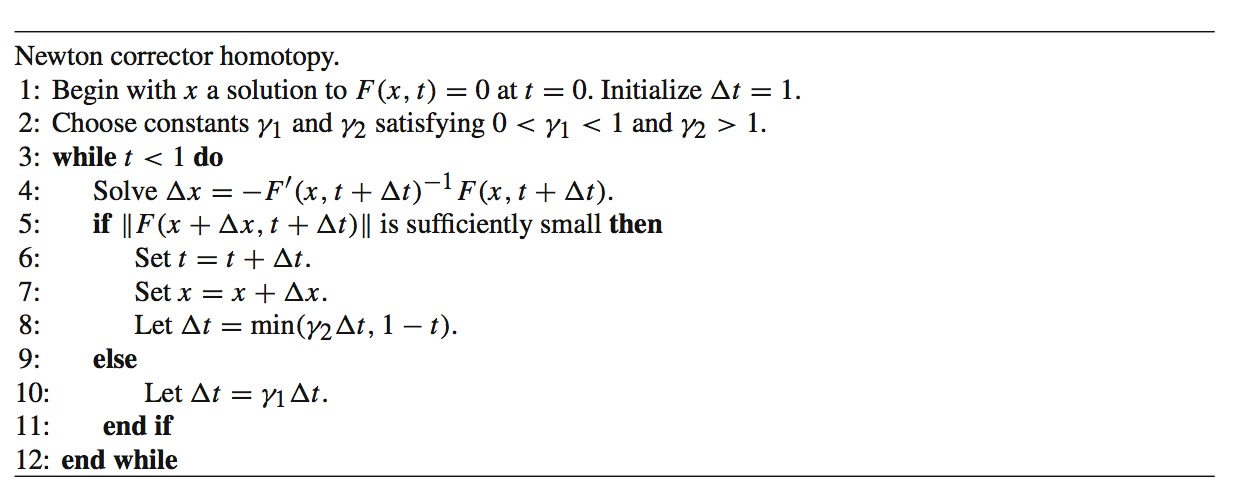
\includegraphics[scale=0.6]{algo_newton_corr}
	
\end{figure}
In this case, there is only a corrector step.
The initial point at which Newton's method is applied is the original $x$.
If $x$ happens to lie in the Newton domain of rapid local convergence for the problem at $t_2$, then the procedure is effective at generating a point that sufficiently contracts $\|F(x,t)\|$ for $t_2-t_2$ small enough that the domain of convergence does not change much.
\par
However, if we include a predictor step, we incorporate first order information in order to estimate the location of the solution at $t_2$.
Here if the first-order estimate is sufficiently accurate, we may take a large step along $t$ and still achieve the desired level of contraction in $\|F\|$ by staying within the domain of local convergence.
The algorithm below uses a canonical predictor-corrector algorithm using one step of a linear tangential predictor and a step of Newton's method.
\begin{figure}[H]
	\centering
	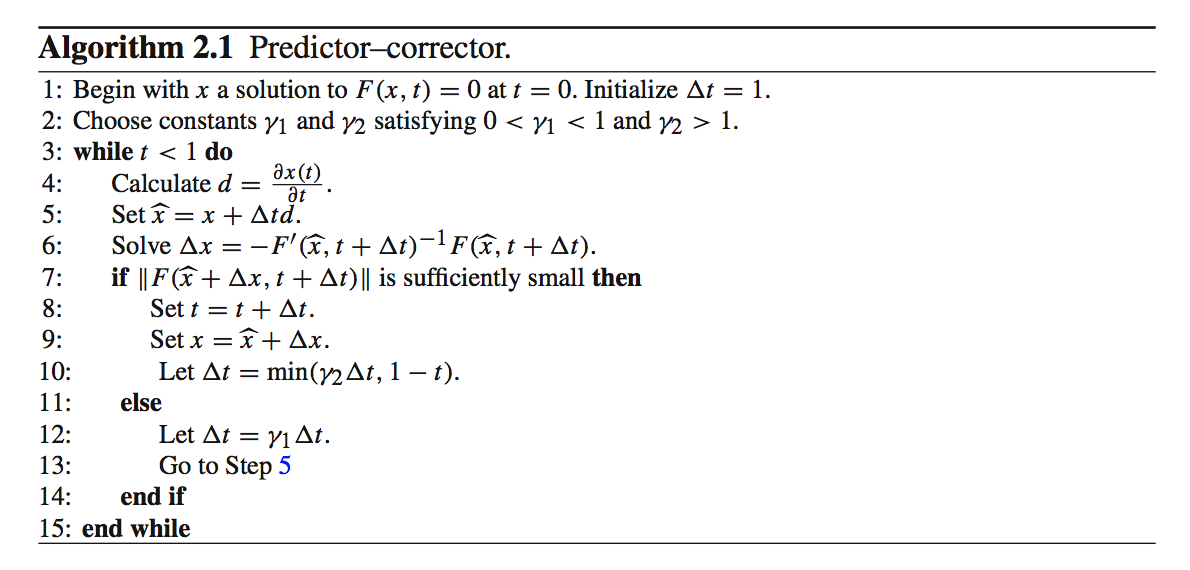
\includegraphics[scale=0.7]{algo_newton_pred_corr}
\end{figure}
This is the Euler-Newton method using exact function and derivative definitions. 
%%%%%%%%%%%%%%%%%%%%%%%%%%%%%%%%%%%%%%%%%%%%%%%%%%%%%%%%%%%%%%%%%%%%%%%
%%%%%%%%%%%%%%%%%%%%%%%%%%%%%%%%%%%%%%%%%%%%%%%%%%%%%%%%%%%%%%%%%%%%%%%
%%%%%%%%%%%%%%%%%%%%%%%%%%%%%%%%%%%%%%%%%%%%%%%%%%%%%%%%%%%%%%%%%%%%%%%
\subsubsection{Predictors for parametric NLP}
In the context of the parametric NLP, the direction of the predictor is the first-order estimate of the change in $x$ and $y$ that would solve the problem corresponding to the change in the parameter $p$.
it also indicates which constraints become inactive with the parameter change.
We shall explore a strategy where a predictor and corrector are computed together in one QP subproblem.
In a general sense, the predictor estimates the newly active or inactive constraints and the corrector refines the step on a properly reduced space with a Newton type iteration.
\par
The directional derivative provides a one-sided estimate of the active set.
In particular, for small perturbations of an NLP, the optimal inactive constraints remain inactive and a subset of the weakly active constraints may become inactive.
The estimation of newly active constraints is done either by linearized constraints at the QP subproblem of the predicted point, or a separate active set estimation procedure.
One estimate of the active set is given by
\begin{equation}
	\mathcal{A}_\gamma(x,y,t)=\{i:c_i(x,t)\leq\eta(x,y,t)^\gamma\}
\end{equation}
where $\gamma$ is a scalar satisfying $0<\gamma<1$.
This estimate is used in the case of the separate predictor and correct step strategy algorithm.
\par
We will now look at the directional differentiability of primal-solution pairs.
Consider a step $(\Delta t,\Delta x,\Delta y)$ for a fixed $\Delta t$ from a base point $(t,\bar{x},\bar{y})$.

\end{document}